%----------------------------------------------------------------------------------------
%	PACKAGES AND DOCUMENT CONFIGURATIONS
%----------------------------------------------------------------------------------------

\documentclass[12pt,a4paper]{article}
\usepackage[margin=1in]{geometry}
\usepackage{graphicx} % Required for the inclusion of images
\usepackage{subfigure} % Required for the inclusion of images
\usepackage{natbib} % Required to change bibliography style to APA
\usepackage{amsmath} % Required for some math elements 
\usepackage{listings}
\usepackage{float} %设置图片浮动位置的宏包
% \usepackage{times} % Uncomment to use the Times New Roman font                     
\usepackage{lstcustom}          
%----------------------------------------------------------------------------------------
%	DOCUMENT INFORMATION
%----------------------------------------------------------------------------------------


\title{\textbf{Project 1: Optimizing the Performance of a Pipelined Processor}} % Title

\author{518030910211\quad Ziqi Zhao\quad bugenzhao@sjtu.edu.cn \\
        518030910188\quad Yimin Zhao\quad doctormin@sjtu.edu.cn \\ } % Author name and email

\date{\today} % Date for the report

\begin{document}

\maketitle % Insert the title, author and date

\section{Introduction}
\textbf{Part A}
\\
In part A, we write three simple assembly programs to implement three functions in \texttt{example.c}. 
Based on ensuring correctness, we especially focus on the functional equivalence with the example C functions. 
By selecting and placing labels in the assembly code appropriately, the code is also very readable.\\ \\
\textbf{Part B}
\\
In part B, we modify the \texttt{HCL} file of the Y86's sequential design to add a new instruction --- \texttt{iaddl}. 
The following is the roadmap to finish this part:
\begin{itemize}
        \item Clarify the computation process of \texttt{iadd} and write it down at the beginning in \texttt{seq-full.hcl}.
        \item Add dependency relations of \texttt{iaddl} to all boolean signals.
        \item Design the datapath for \texttt{iaddl}, i.e., generate control signals for \texttt{src} and \texttt{dst}
\end{itemize}
\textbf{Part C}
\\
We achieve full scores in the benchmark testing \textbf{in just 2 hours}, 
but we \textbf{spent 2 more days} researching all the potential methods to optimize the performance even further. 
The following is our roadmap:
\begin{itemize}
        \item Change the order of the instruction sequence to avoid data hazard and structure hazards as much as possible, which leaves $CPE = 12.96$.
        \item Beyond the changes on instruction order, we apply loop unrolling to reduce the number of conditional check and registers updating, which leaves $CPE = 9.83$.
        \item Use a binary search tree to find the precise remaining number of elements after several rounds of unrolling to achieve complete unrolling, which leaves $CPE = 8.95$.
        \item Modify the pipeline design in \texttt{HCL} file to achieve 100\% accuracy in branch prediction for certain code pattern, which {\color{blue}\textbf{brings $\mathbf{CPE}$ down to $\mathbf{7.79}$}}.
\end{itemize}
\textbf{Contribution}
\begin{itemize}
	\item \textbf{Ziqi Zhao} : Part A (coding) \& Part B (coding) \& Part C (coding \& designing) \& project report (reviewing)
	\item \textbf{Yimin Zhao} : Part A (reviewing \& coding) \& Part B (reviewing) \& Part C (designing) \& project report (writing)
\end{itemize}
\
\textbf{Special Notes for Testing the Part C}
\begin{itemize}
	\item In the Part C, we first achieved full marks by simply adding the \texttt{iaddl} instruction to \texttt{HCL} file, and in an almost software-only way. The hardware implementation of this approach is in \texttt{pipe-full.hcl}.
	\item After that, we made a further exploration and made a modification to the branch prediction part, and finally achieved a CPE of $7.79$. {\color{blue}The hardware implementation of this approach is in \texttt{pipe-zzcc.hcl}.}
\end{itemize}
\pagebreak
\section{Experiments}
\subsection{Part A}
\subsubsection{Analysis}
In this part, we are asked to implement and simulate three Y86 programs. 
From a macro point of view, this part is relatively easy. 
But there are plenty of optimizations worth exploring in terms of code readability and elegance.\\\\
\textbf{Difficult Point} 
\begin{itemize}
        \item Always pull the correct element from the stack.
        \item Be careful to protect the callee-saved register: \texttt{EBX, EDI, ESI}.
        \item Implement function recursion smartly.
\end{itemize}
\textbf{Core Technique}
\begin{itemize}
        \item Mimicking C functions, division of functional areas with enough and clear label.
        \item Get the fastest completion speed by coding line by line referring to C language functions.
        \item Always draw a picture of the stack to ensure the correctness of fetching a variable.
\end{itemize}

\subsubsection{Code}
\begin{center}
        \textbf{sum.ys}
\end{center}

\begin{lstlisting}
# 518030910211 ZiqiZhao
# 518030910188 YiminZhao

    .pos    0
main:
    irmovl  stack, %esp     # initialize stack
    rrmovl  %esp, %ebp      # initialize frame
    irmovl  ele1, %eax
    pushl   %eax            # argument
    call    sum_list
    halt

# Sample linked list 
.align 4
ele1:
    .long   0x00a
    .long   ele2
ele2:
    .long   0x0b0
    .long   ele3
ele3:
    .long   0xc00
    .long   0

# sum_list func
sum_list:
    pushl   %ebp            # enter
    rrmovl  %esp, %ebp
    xorl    %eax, %eax      # clear %eax
    mrmovl  8(%ebp), %edx   # %edx = ls
    jmp     test
loop:
    mrmovl  (%edx), %ecx    # tmp = ls->val
    addl    %ecx, %eax      # val += tmp
    mrmovl  4(%edx), %edx   # ls = ls->next
test:
    andl    %edx, %edx      # ls == 0?
    jne     loop            # no -> loop
return:
    rrmovl  %ebp, %esp      # leave
    popl    %ebp
    ret


# Stack 
    .pos    0x400
stack:

\end{lstlisting}
\begin{center}
        \textbf{rsum.ys}
\end{center}
\begin{lstlisting}
# 518030910211 ZiqiZhao
# 518030910188 YiminZhao

# Set up stack
    .pos    0
    irmovl  stack, %esp
    rrmovl  %esp, %ebp
    irmovl  ele1, %eax
    pushl   %eax
    call    rsum_list
    halt

# Sample linked list 
.align 4
ele1:
    .long   0x00a
    .long   ele2
ele2:
    .long   0x0b0
    .long   ele3
ele3:
    .long   0xc00
    .long   0

# rsum_list func
rsum_list:
    pushl   %ebp            # enter
    rrmovl  %esp, %ebp
    pushl   %ebx            # save %ebx
    xorl    %eax, %eax      # clear eax
    mrmovl  8(%ebp), %edx   # get ls
    andl    %edx, %edx      # ls == NULL?
    je      return          # yes -> return
do:
    mrmovl  (%edx), %ebx    # mov ls->val to %ebx
    mrmovl  4(%edx), %eax
    pushl   %eax            # push ls->next
    call    rsum_list
    addl    %ebx, %eax      # ret = val + ret
    popl    %edx            # eat para
return:
    popl    %ebx            # restore %ebx
    rrmovl  %ebp, %esp      # leave
    popl    %ebp
    ret


# Stack 
    .pos    0x400
stack:
\end{lstlisting}
\begin{center}
        \textbf{copy.ys}
\end{center}
\begin{lstlisting}
# 518030910211 ZiqiZhao
# 518030910188 YiminZhao

# Set up stack
    .pos    0
    irmovl  stack, %esp
    rrmovl  %esp, %ebp
    irmovl  $3, %eax        # len
    pushl   %eax
    irmovl  dest, %eax      # dest
    pushl   %eax
    irmovl  src, %eax       # src
    pushl   %eax
    call    copy_block
    halt

.align 4
# Source block
src:
    .long 0x00a
    .long 0x0b0
    .long 0xc00
    .long 0x888             # Should not copy this

# Destination block
dest:
    .long 0x111
    .long 0x222
    .long 0x333
    .long 0x999             # Should not write this

copy_block:
    pushl   %ebp            # enter
    rrmovl  %esp, %ebp
    pushl   %ebx            # save %ebx -> len
    pushl   %edi            # save %edi -> immediate
    pushl   %esi            # save %esi -> val
    xorl    %eax, %eax      # %eax = result = 0
    mrmovl  16(%ebp), %ebx  # %ebx = len
    mrmovl  12(%ebp), %edx  # %edx = dest
    mrmovl  8(%ebp), %ecx   # %ecx = src
    jmp     test
loop:
    irmovl  $4, %edi        # %edi = 4
    mrmovl  (%ecx), %esi    # val = *src
    addl    %edi, %ecx      # src += 1
    rmmovl  %esi, (%edx)    # *dest = val
    addl    %edi, %edx      # val += 1
    xorl    %esi, %eax      # result ^= val
    irmovl  $-1, %edi       # %edx = -1
    addl    %edi, %ebx      # len -= 1
test:
    andl    %ebx, %ebx      # len > 0?
    jg      loop            # yes -> loop
return:
    popl    %esi            # restore registers
    popl    %edi
    popl    %ebx
    rrmovl  %ebp, %esp      # leave
    popl    %ebp
    ret
# Stack 
    .pos    0x400
stack:
\end{lstlisting}

\subsubsection{Evaluation}
\begin{itemize}
	\item \textbf{sum.ys}\\

\begin{figure}[H] %H为当前位置,!htb为忽略美学标准,htbp为浮动图形
        \centering %图片居中
        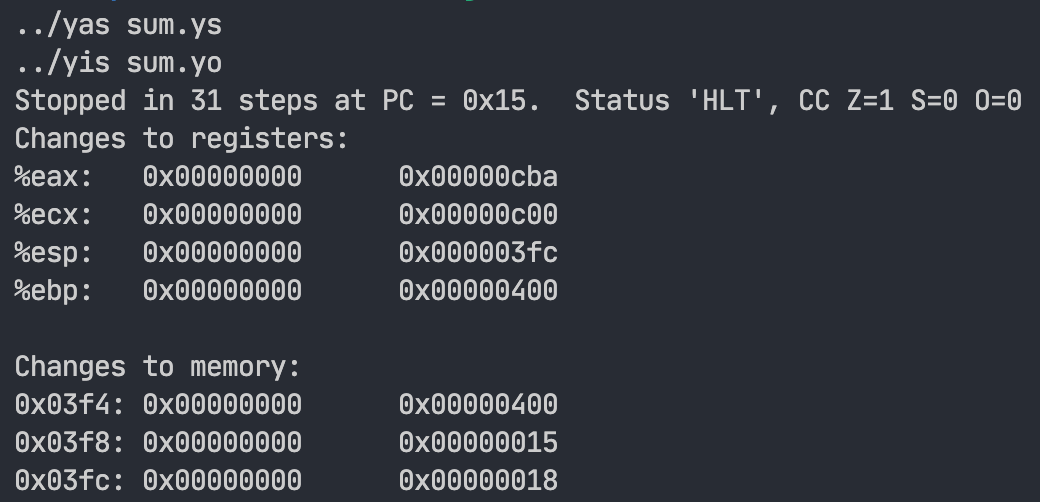
\includegraphics[width=0.7\textwidth]{partA-sum-bz.png} %插入图片,[]中设置图片大小,{}中是图片文件名
        \caption{Part A: sum.ys} %最终文档中希望显示的图片标题
        \label{Fig.partA-sum} %用于文内引用的标签
\end{figure}
\begin{itemize}
        \item The \texttt{\%eax} register has the correct value which is the return value of the function --- \texttt{0xcba}.
        \item The memory is not corrupted since all the modifications locate at the stack whose starting addresss is set to be \texttt{0x400}.
\end{itemize}
	\item \textbf{rsum.ys}\\

\begin{figure}[H] %H为当前位置,!htb为忽略美学标准,htbp为浮动图形
        \centering %图片居中
        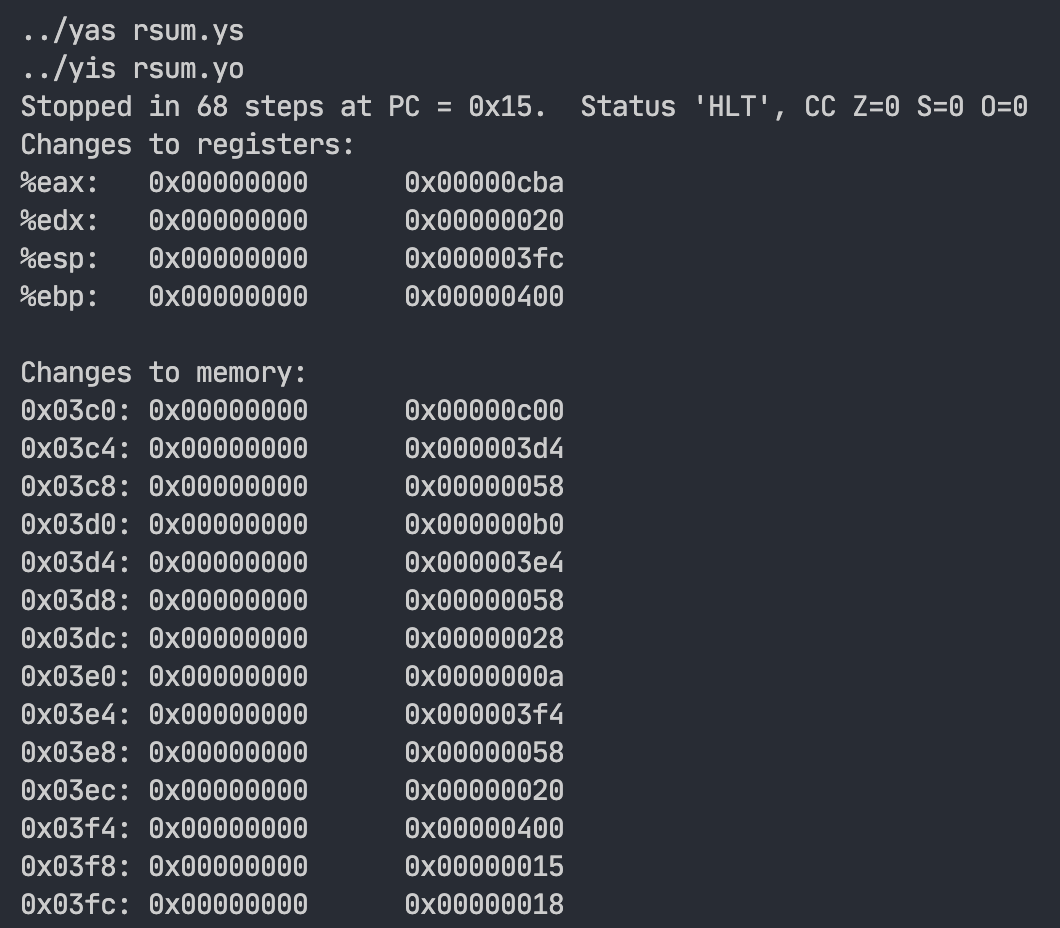
\includegraphics[width=0.61\textwidth]{partA-rsum-bz.png} %插入图片,[]中设置图片大小,{}中是图片文件名
        \caption{Part A: rsum.ys} %最终文档中希望显示的图片标题
        \label{Fig.partA-rsum} %用于文内引用的标签
\end{figure}

\begin{itemize}
        \item The \texttt{\%eax} register has the correct value which is the return value of the function --- \texttt{0xcba}.
        \item The memory is not corrupted since all the modifications locate at the stack whose starting addresss is set to be \texttt{0x400}.
\end{itemize}

	\item \textbf{copy.ys}\\

\begin{figure}[H] %H为当前位置,!htb为忽略美学标准,htbp为浮动图形
        \centering %图片居中
        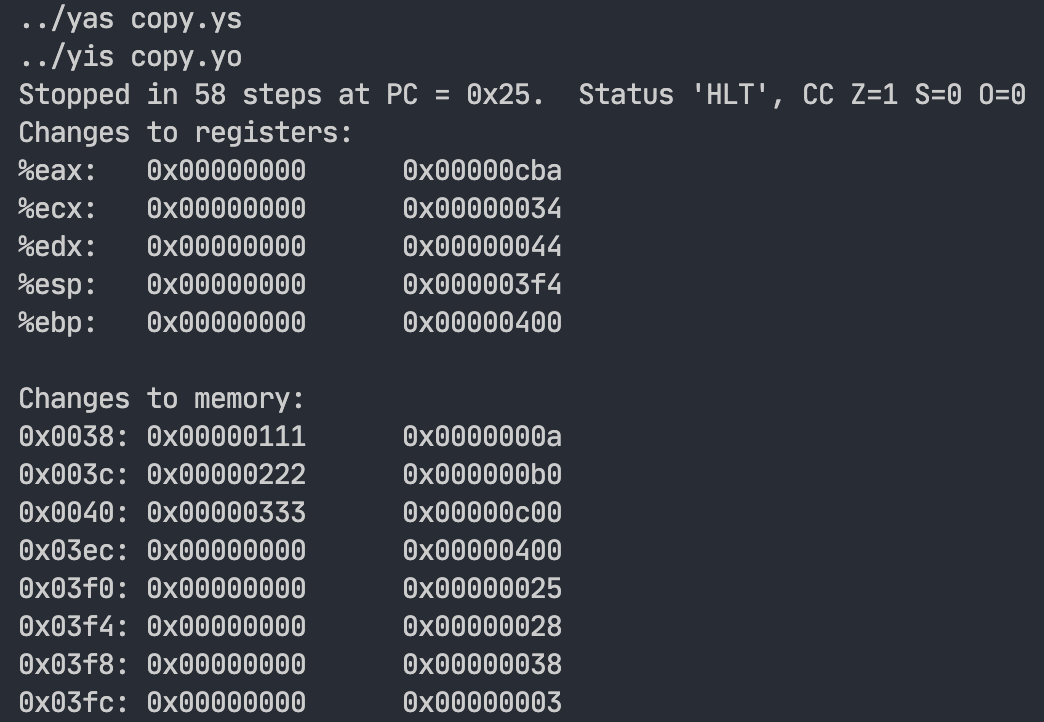
\includegraphics[width=0.7\textwidth]{partA-copy-bz.png} %插入图片,[]中设置图片大小,{}中是图片文件名
        \caption{Part A: copy.ys} %最终文档中希望显示的图片标题
        \label{Fig.partA-copy} %用于文内引用的标签
\end{figure}

\begin{itemize}
        \item The \texttt{\%eax} register has the correct value which is the return value of the function --- \texttt{0xcba}.
        \item Values are written into the memory correctly as shown in the first three rows in the "Changes to memory" part in Figure 3.
        \item The memory is not corrupted since all the modifications other than \texttt{dest} locate at the stack whose starting addresss is set to be \texttt{0x400}.
\end{itemize}
\end{itemize}
\pagebreak
\subsection{Part B}

\subsubsection{Analysis}
In part B, we are asked to extend the SEQ processor to support instruction \texttt{iaddl} by modifying \texttt{SEQ-full.hcl}.
The task is not so difficult once we understand the processing logic and the syntax of \texttt{HCL}, and all we need to do is change the followings in \texttt{seq-full.hcl}:
\begin{itemize}
        \item Add \texttt{IIADDL} in the choices region of \texttt{(bool) instr\_valid} since \texttt{iaddl} is a valid instruction.
        \item Add \texttt{IIADDL} in the choices region of \texttt{(bool) need\_regid} since \texttt{iaddl} operation involves one register.
        \item Add \texttt{IIADDL} in the choices region of \texttt{(bool) need\_valC} since \texttt{iaddl} operation involves one constant (represented by \texttt{valC} in the circult of Y86 SEQ).
        \item Add \texttt{IIADDL} in the choices region of \texttt{(bool) set\_cc} since \texttt{iaddl} operation involves ALU operation which will set flags.
        \item When icode is \texttt{IIADDL}, \texttt{alufun} will be \texttt{ALUADD} since the operation is "adding" the constant to \texttt{rB}.
        \item When icode is \texttt{IIADDL}, \texttt{srcB} is from \texttt{rB} since the second operand of \texttt{iaddl} is a register.
        \item When icode is \texttt{IIADDL}, \texttt{dstE} (where the result from ALU is passed towards) is \texttt{rB} since "\texttt{iaddl constant, rB}" means \texttt{rB += constant} (\texttt{rB} is updated). 
        \item When icode is \texttt{IIADDL}, \texttt{aluA} (the first op) is \texttt{valC} (the constant in the instruction) since "\texttt{iaddl constant, rB}" means the first op is the constant (\texttt{valC}).
        \item When icode is \texttt{IIADDL}, \texttt{aluB} (the second op) is \texttt{valB} (the value of the second register that is read) for the same reason above.
\end{itemize}

\subsubsection{Code}
\begin{center}
        \textbf{Modifications in SEQ-full.hcl}
\end{center}
\begin{lstlisting}
--------------------------------------------------------------------
bool instr_valid = icode in 
     { INOP, IHALT, IRRMOVL, IIRMOVL, IRMMOVL, IMRMOVL,
       IOPL, IJXX, ICALL, IRET, IPUSHL, IPOPL, IIADDL };
--------------------------------------------------------------------
# Does fetched instruction require a regid byte?
bool need_regids =
        icode in { IRRMOVL, IOPL, IPUSHL, IPOPL, 
                IIRMOVL, IRMMOVL, IMRMOVL, IIADDL };
--------------------------------------------------------------------
# Does fetched instruction require a constant word?
bool need_valC =
        icode in { IIRMOVL, IRMMOVL, IMRMOVL, IJXX, ICALL, IIADDL };
--------------------------------------------------------------------
## What register should be used as the B source?
int srcB = [
        icode in { IOPL, IRMMOVL, IMRMOVL, IIADDL  } : rB;
        icode in { IPUSHL, IPOPL, ICALL, IRET } : RESP;
        1 : RNONE;  # Don't need register
];
--------------------------------------------------------------------
## What register should be used as the E destination?
int dstE = [
        icode in { IRRMOVL } && Cnd : rB;
        icode in { IIRMOVL, IOPL, IIADDL } : rB;
        icode in { IPUSHL, IPOPL, ICALL, IRET } : RESP;
        1 : RNONE;  # Don't write any register
];
--------------------------------------------------------------------
## Select input A to ALU
int aluA = [
        icode in { IRRMOVL, IOPL } : valA;
        icode in { IIRMOVL, IRMMOVL, IMRMOVL, IIADDL } : valC;
        icode in { ICALL, IPUSHL } : -4;
        icode in { IRET, IPOPL } : 4;
        # Other instructions don't need ALU
];
--------------------------------------------------------------------
## Select input B to ALU
int aluB = [
        icode in { IRMMOVL, IMRMOVL, IOPL, ICALL, 
                IPUSHL, IRET, IPOPL, IIADDL } : valB;
        icode in { IRRMOVL, IIRMOVL } : 0;
        # Other instructions don't need ALU
];
--------------------------------------------------------------------
## Set the ALU function
int alufun = [
        icode == IOPL : ifun;
        icode == IIADDL : ALUADD;
        1 : ALUADD;
];
--------------------------------------------------------------------
## Should the condition codes be updated?
bool set_cc = icode in { IOPL, IIADDL };
--------------------------------------------------------------------
\end{lstlisting}
\subsubsection{Evaluation}
\begin{figure}[H] %H为当前位置,!htb为忽略美学标准,htbp为浮动图形
        \centering %图片居中
        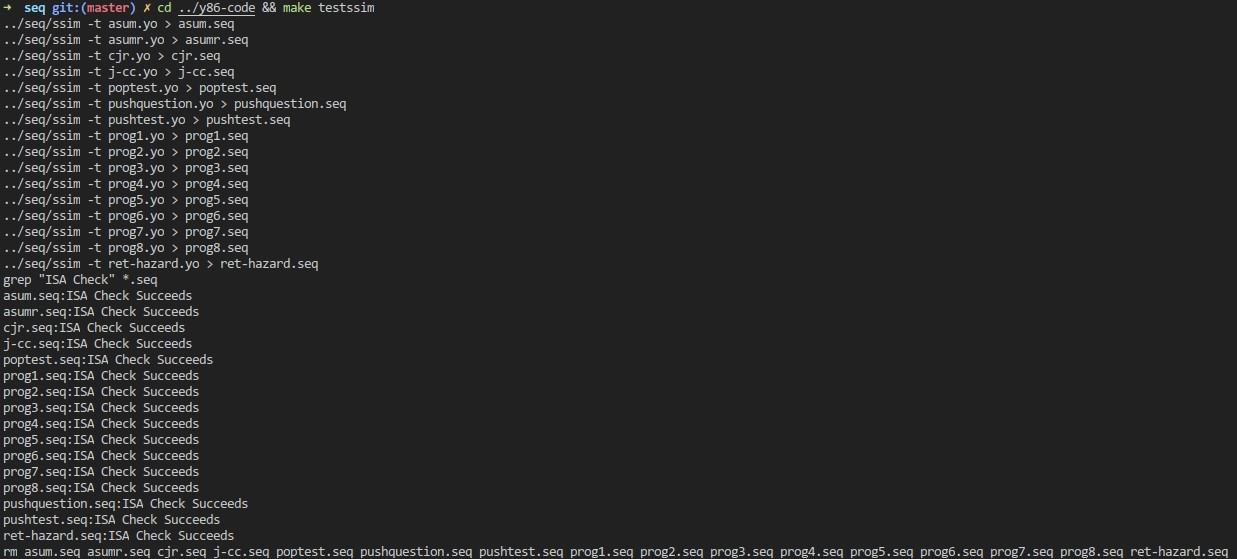
\includegraphics[width=1.0\textwidth]{partB-benchmark.jpg} %插入图片,[]中设置图片大小,{}中是图片文件名
        \caption{Part B: benchmark test} %最终文档中希望显示的图片标题
        \label{Fig.partB-benchmark} %用于文内引用的标签
\end{figure}
\begin{figure}[H] %H为当前位置,!htb为忽略美学标准,htbp为浮动图形
        \centering %图片居中
        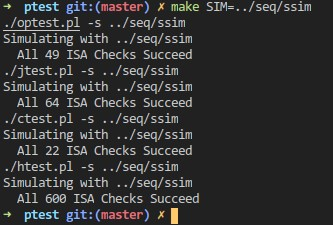
\includegraphics[width=0.6\textwidth]{partB-regression-test.jpg} %插入图片,[]中设置图片大小,{}中是图片文件名
        \caption{Part B: regression test} %最终文档中希望显示的图片标题
        \label{Fig.partB-regression} %用于文内引用的标签
\end{figure}
\begin{figure}[H] %H为当前位置,!htb为忽略美学标准,htbp为浮动图形
        \centering %图片居中
        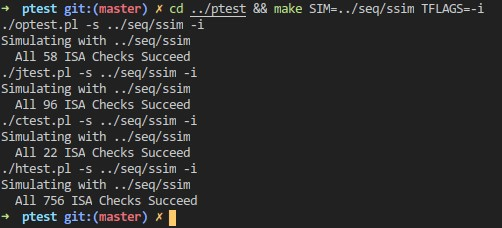
\includegraphics[width=0.6\textwidth]{partB-test-iaddl.jpg} %插入图片,[]中设置图片大小,{}中是图片文件名
        \caption{Part B: \texttt{iaddl} test} %最终文档中希望显示的图片标题
        \label{Fig.partB-iaddl} %用于文内引用的标签
\end{figure}
\pagebreak
\subsection{Part C}
\subsubsection{Analysis}
In this part, we were asked to speed up the program \texttt{ncopy.ys} as much as possible by modifying the \texttt{ncopy.ys} and \texttt{HCL}.
The following is our roadmap:\\
\\
\textbf{Added \texttt{iaddl} instruction to \texttt{pipe-full.hcl} }

Like what we have done in Part B, we added \texttt{iaddl} to the pipeline design. It avoided the overhead of using registers to store constants, and also increased the number of registers we could use, which paved the way for our further optimization.\\
\\
\textbf{Avoid Load and Use: CPE $\rightarrow$ 12.96}

For the pipeline design in CS:APP 2e, "load and use" or \texttt{mrmovl} then \texttt{rmmovl} will cause penalty,
which must be avoided to improve the performance. On the one hand, we rearranged the order of 
instructions to avoid stalling as much as possible. On the other hand, we use two registers to store 
the variable \texttt{val}, loading them separately and ahead of time.\\
\\
\textbf{10-way Loop Unrolling:  CPE $\rightarrow$ 9.83}

There's much overhead in testing and updating procedure of loops, and one way to minimize it is to 
perform a technique named "loop unrolling". That is, we do multiple loops and update the relevant 
data at once, to reduce the number of times we execute the \texttt{add} and \texttt{jxx} instructions. \\
\\
\textbf{Search Tree for Remaining Elements:  CPE $\rightarrow$ 8.95}

For large inputs, the more ways we unroll the loops, the better the program performs. However, for 
small inputs, it is important to choose a good method to process the remaining elements. The simplest 
way is to write another loop for them, but a much better way is to totally unroll the code, that is, 
jump to different position for different number of remaining ones. Since Y86 does not support relative 
jump instruction, we designed a search tree to get the correct jump destination for each possibility.
\\
\\
--------------------------------------------------------------------------------------------------------\\
The above optimization took us two hours, so far we have reached full marks.\\
\textbf{But can it be even faster?}
We spent another two days poring over the implementation logic in \texttt{HCL} and other files of the Y86 pipeline design. And it finally got us here:\\
--------------------------------------------------------------------------------------------------------\\
\\
{\color{red}\textbf{Optimized for Our Branch Prediction Design: CPE $\rightarrow$ 7.79}} 

For this program, a significant performance factor is the branch prediction failure for \texttt{count++}.
In \texttt{pipe-zzcc.hcl}, we made a special optimization for the situation like this:
\begin{center}

\begin{tabular}{|c|c|c|c|}
        \hline Instruction&any instruction&non-alu instruction&\texttt{jxx}\\
        \hline Stages&EX&ID&IF\\
        \hline
\end{tabular}
\end{center}

Note that in this case, we can forward the conditions from EX stage to IF and predict the branch with 100\% accuracy. 
Thus, we optimized the program to ensure that there were as many of these patterns as 
possible and took much advantage of it, which leads to an average CPE of 7.79.
\subsubsection{Code}
\begin{center}
        \textbf{-----10-Way Loop Unrolling-----}\\
\end{center}
\begin{lstlisting}
##################################################################
# You can modify this portion
# Entry
	iaddl $-9, %edx		# len -= 9, i.e., initial_len <= 9?
	irmovl $0, %eax		# count = 0
	jle Remaining		# if so, goto Remaining

# Loop unrolling part
Loop0:	
	mrmovl (%ebx), %esi	# valA = src[0]
	mrmovl 4(%ebx), %edi	# valB = src[1]
	andl %esi, %esi		# valA <= 0?
	rmmovl %esi, (%ecx)	# dst[0] = valA
	jle Loop1		# if so, goto next loop
	iaddl $1, %eax		# count++
Loop1:	
	mrmovl 8(%ebx), %esi	# valA = src[2]
	andl %edi, %edi		# valB <= 0?
	rmmovl %edi, 4(%ecx)	# dst[1] = valB
	jle Loop2		# if so, goto next loop
	iaddl $1, %eax		# count++
Loop2:
	mrmovl 12(%ebx), %edi	# valB = src[3]
	andl %esi, %esi		# valA <= 0?
	rmmovl %esi, 8(%ecx)	# dst[2] = valA
	jle Loop3		# if so, goto next loop
	iaddl $1, %eax		# count++
Loop3:	
	mrmovl 16(%ebx), %esi	# valA = src[4]
	andl %edi, %edi		# valB <= 0?
	rmmovl %edi, 12(%ecx)	# dst[3] = valB
	jle Loop4		# if so, goto next loop
	iaddl $1, %eax		# count++
Loop4:
	mrmovl 20(%ebx), %edi	# valB = src[5]
	andl %esi, %esi		# valA <= 0?
	rmmovl %esi, 16(%ecx)	# dst[4] = valA
	jle Loop5		# if so, goto next loop
	iaddl $1, %eax		# count++
Loop5:	
	mrmovl 24(%ebx), %esi	# valA = src[6]
	andl %edi, %edi		# valB <= 0?
	rmmovl %edi, 20(%ecx)	# dst[5] = valB
	jle Loop6		# if so, goto next loop
	iaddl $1, %eax		# count++
Loop6:
	mrmovl 28(%ebx), %edi	# valB = src[7]
	andl %esi, %esi		# valA <= 0?
	rmmovl %esi, 24(%ecx)	# dst[6] = valA
	jle Loop7		# if so, goto next loop
	iaddl $1, %eax		# count++
Loop7:	
	mrmovl 32(%ebx), %esi	# valA = src[8]
	andl %edi, %edi		# valB <= 0?
	rmmovl %edi, 28(%ecx)	# dst[7] = valB
	jle Loop8		# if so, goto next loop
	iaddl $1, %eax		# count++
Loop8:
	mrmovl 36(%ebx), %edi	# valB = src[9]
	andl %esi, %esi		# valA <= 0?
	rmmovl %esi, 32(%ecx)	# dst[8] = valA
	jle Loop9		# if so, goto next loop
	iaddl $1, %eax		# count++
Loop9:
	andl %edi, %edi		# valB <= 0?
	rmmovl %edi, 36(%ecx)	# dst[9] = valB
	jle LoopEnd		# if so, goto loop end
	iaddl $1, %eax
LoopEnd:
	iaddl $40, %ecx		# dst += 10 * 4
	iaddl $40, %ebx		# src += 10 * 4
	iaddl $-10, %edx	# len -= 10
	jg Loop0		# if so, goto Loop0
                                # else, goto process remaining elements
\end{lstlisting}

\begin{center}
        \textbf{-----Binary Search Tree for Finding the Number of Remaining Loops-----}\\
\end{center}
\begin{lstlisting}
# The following block is a binary search tree to 
# find the number of remaining loops 
# (which must be less than 10) at minimal cost
Remaining:
	iaddl $6, %edx		# [-9,0] -> [-3,6]	(+3)
RemTest:
	irmovl $0, %esi
	jg RemTestR
	je Rem3
RemTestL:
	iaddl $2, %edx		# [-3,-1] -> [-1,1]	(+1)
	je Rem1
	jg Rem2
	jmp Done		# -1 + 1 = 0
RemTestR:
	iaddl $-3, %edx		# [1,6] -> [-2,3]	(+6)
	jg RemTestRR
	je Rem6
RemTestRL:
	iaddl $1, %edx		# [-2,-1] -> [-1,0]	(+5)
	jl Rem4
	je Rem5
RemTestRR:
	iaddl $-2, %edx		# [1,3] -> [-1,1]	(+8)
	jl Rem7
	je Rem8
\end{lstlisting}

\begin{center}
        \textbf{-----Unrolling of Remaining Loops-----}\\
\end{center}
\begin{lstlisting}
Rem9:
	mrmovl 32(%ebx), %esi	# valA = src[8]
	rmmovl %esi, 32(%ecx)	# dst[8] = valA
Rem8:	# Note that %esi == 0, directly jumping here
	#  implies that RemXb will performs correctly.
	andl %esi, %esi		# valA <= 0?
	mrmovl 28(%ebx), %esi	# valA = src[7]
	jle Rem8b		# if so, goto Rem8b
	iaddl $1, %eax		# count++
Rem8b:	rmmovl %esi, 28(%ecx)	# dst[7] = valA
Rem7:	
	andl %esi, %esi		# valA <= 0?
	mrmovl 24(%ebx), %esi	# valA = src[6]
	jle Rem7b		# if so, goto Rem7b
	iaddl $1, %eax		# count++
Rem7b:	rmmovl %esi, 24(%ecx)	# dst[6] = valA
Rem6:	
	andl %esi, %esi		# valA <= 0?
	mrmovl 20(%ebx), %esi	# valA = src[5]
	jle Rem6b		# if so, goto Rem6b
	iaddl $1, %eax		# count++
Rem6b:	rmmovl %esi, 20(%ecx)	# dst[5] = valA
Rem5:	
	andl %esi, %esi		# valA <= 0?
	mrmovl 16(%ebx), %esi	# valA = src[4]
	jle Rem5b		# if so, goto Rem5b
	iaddl $1, %eax		# count++
Rem5b:	rmmovl %esi, 16(%ecx)	# dst[4] = valA
Rem4:	
	andl %esi, %esi		# valA <= 0?
	mrmovl 12(%ebx), %esi	# valA = src[3]
	jle Rem4b		# if so, goto Rem4b
	iaddl $1, %eax		# count++
Rem4b:	rmmovl %esi, 12(%ecx)	# dst[3] = valA
Rem3:	
	andl %esi, %esi		# valA <= 0?
	mrmovl 8(%ebx), %esi	# valA = src[2]
	jle Rem3b		# if so, goto Rem3b
	iaddl $1, %eax		# count++
Rem3b:	rmmovl %esi, 8(%ecx)	# dst[2] = valA
Rem2:	
	andl %esi, %esi		# valA <= 0?
	mrmovl 4(%ebx), %esi	# valA = src[1]
	jle Rem2b		# if so, goto Rem2b
	iaddl $1, %eax		# count++
Rem2b:	rmmovl %esi, 4(%ecx)	# dst[1] = valA
Rem1:	
	andl %esi, %esi		# valA <= 0?
	mrmovl (%ebx), %esi	# valA = src[0]
	jle Rem1b		# if so, goto Rem1b
	iaddl $1, %eax		# count++
Rem1b:	
	andl %esi, %esi		# valA <= 0?
	rmmovl %esi, (%ecx)	# dst[0] = valA
	jle Done		# if so, goto Done
        iaddl $1, %eax		# count++
        
\end{lstlisting}
\begin{center}
        {\color{blue}\textbf{-----Modification to \texttt{hcl} (all in \texttt{pipe-zzcc.hcl})-----}}\\
        Note: here we have omitted the changes for adding \texttt{iaddl}, \\which is the same as those in \texttt{seq-full.hcl} and \texttt{pipe-full.hcl}
\end{center}
\begin{lstlisting} 
# 1. Added instruction `iaddl`
#   Similar to the changes in `../seq/full.hcl`.
#
# 2. Optimization on branch prediction
#   a. For unconditional JMP, there's no need to insert any bubble.
#
#   b. A significant performance factor is the branch prediction failure for count++. In our design, we made a special optimization for the situation like this:
#         Instruction:   any    non-alu    jxx
#         Stage:         EX       ID       IF
#      Note that in this case, we can forward the conditions from EX stage to IF and predict the branch with 100% accuracy. Thus, we optimized the program to ensure that there were as many of these patterns as possible and took much advantage of it, which leads to an average CPE of 7.79.
#
#      Specifically, we have modified the following logic:
#     - Added some additional definitions around line 150;
#     - Modified SelectPC logic around line 180;
#     - Modified PredictPC logic around line 230;
#     - Modified pipeline bubble logic around line 400 and 410.

---------------------Added following definition-----------------------
quote 'int gen_aluA();'			# Declaration of gen_aluA
quote 'int gen_aluB();'			# Declaration of gen_aluB

# For JXX in ID and ALU in EX, check the cc generated by ALU
# Note that the simulator do not generate `cc_in` correctly
boolsig f_cnd_alu 
        'cond_holds(compute_cc(id_ex_curr->ifun, 
                    gen_aluA(), gen_aluB()), 
                    if_id_next->ifun)'

# For JXX in ID and non-ALU in EX, check the cc register
boolsig f_cnd_other 'cond_holds(cc, if_id_next->ifun)'

---------------------------Modified f_PC------------------------------
## What address should instruction be fetched at
int f_pc = [
	# Unconditional jump: Use predicted value of PC
	M_icode == IJXX && M_ifun == UNCOND : F_predPC;

	# Mispredicted taken. Fetch at incremented PC (previously valP)
	M_icode == IJXX && (W_icode in {IOPL, IIADDL}) && !M_Cnd : M_valA;

	# Completion of RET instruction.
	W_icode == IRET : W_valM;

	# Default: Use predicted value of PC
	1 : F_predPC;
];

-------------------------Modified f_predPC----------------------------
# Predict next value of PC
int f_predPC = [
	f_icode == ICALL : f_valC;
	f_icode == IJXX && f_ifun == UNCOND : f_valC;

	# Decode stage is ALU and will set CC->always taken by default
	f_icode == IJXX && (D_icode in {IOPL, IIADDL}): f_valC;

	# Decode stage is not ALU
	 # Execute stage is ALU -> compute CC
        f_icode == IJXX && (E_icode in {IOPL, IIADDL}) && 
        !f_cnd_alu : f_valP;

	 # Execute stage is not ALU -> check cc -> ZF SF OF
        f_icode == IJXX && !(E_icode in {IOPL, IIADDL}) && 
        !f_cnd_other : f_valP;
        
        # Other JXX
	f_icode == IJXX : f_valC;

	# Otherwise
	1 : f_valP;
];

---------------Added conditions to D_Bubble & E_BUbble----------------
bool D_bubble =
	# Mispredicted branch taken
        (E_icode == IJXX && E_ifun != UNCOND && 
        (M_icode in {IOPL, IIADDL}) && !e_Cnd) ||
	# Stalling at fetch while ret passes through pipeline
	# but not condition for a load/use hazard
        !(E_icode in { IMRMOVL, IPOPL } 
        && E_dstM in { d_srcA, d_srcB }) 
        && IRET in { D_icode, E_icode, M_icode };


bool E_bubble =
	# Mispredicted branch taken
        (E_icode == IJXX && E_ifun != UNCOND && 
        (M_icode in {IOPL, IIADDL}) && !e_Cnd) ||
	# Conditions for a load/use hazard
	E_icode in { IMRMOVL, IPOPL } &&
	 E_dstM in { d_srcA, d_srcB};
\end{lstlisting}
\subsubsection{Evaluation}
Note: both designs in \texttt{pipe-full.hcl} and \texttt{pipe-zzcc.hcl} have passed the tests and got full marks. Considering that the latter is a superset of the former, we have omitted the test screenshots of \texttt{pipe-full.hcl} here. The following results are the latter one's.
\begin{figure}[H] %H为当前位置,!htb为忽略美学标准,htbp为浮动图形
        \centering %图片居中
        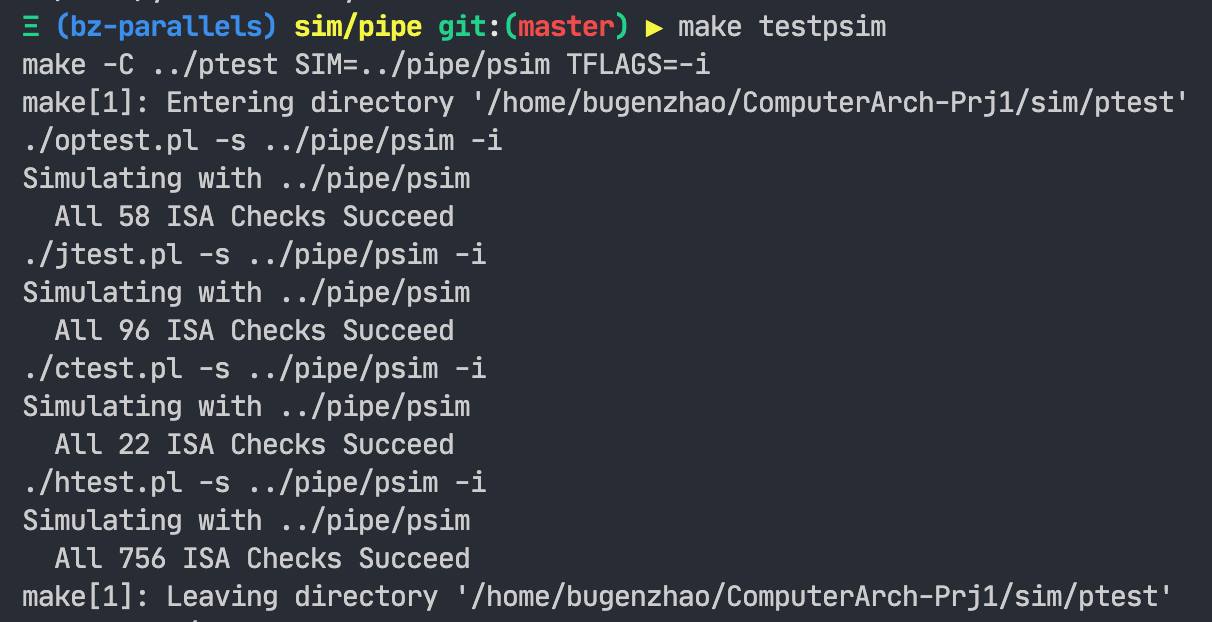
\includegraphics[width=0.7\textwidth]{partC-regression-test.png} %插入图片,[]中设置图片大小,{}中是图片文件名
        \caption{Part C: regression test (with \texttt{iaddl} included)} %最终文档中希望显示的图片标题
        \label{Fig.partC-regression} %用于文内引用的标签
\end{figure}
\begin{figure}[H] %H为当前位置,!htb为忽略美学标准,htbp为浮动图形
        \centering %图片居中
        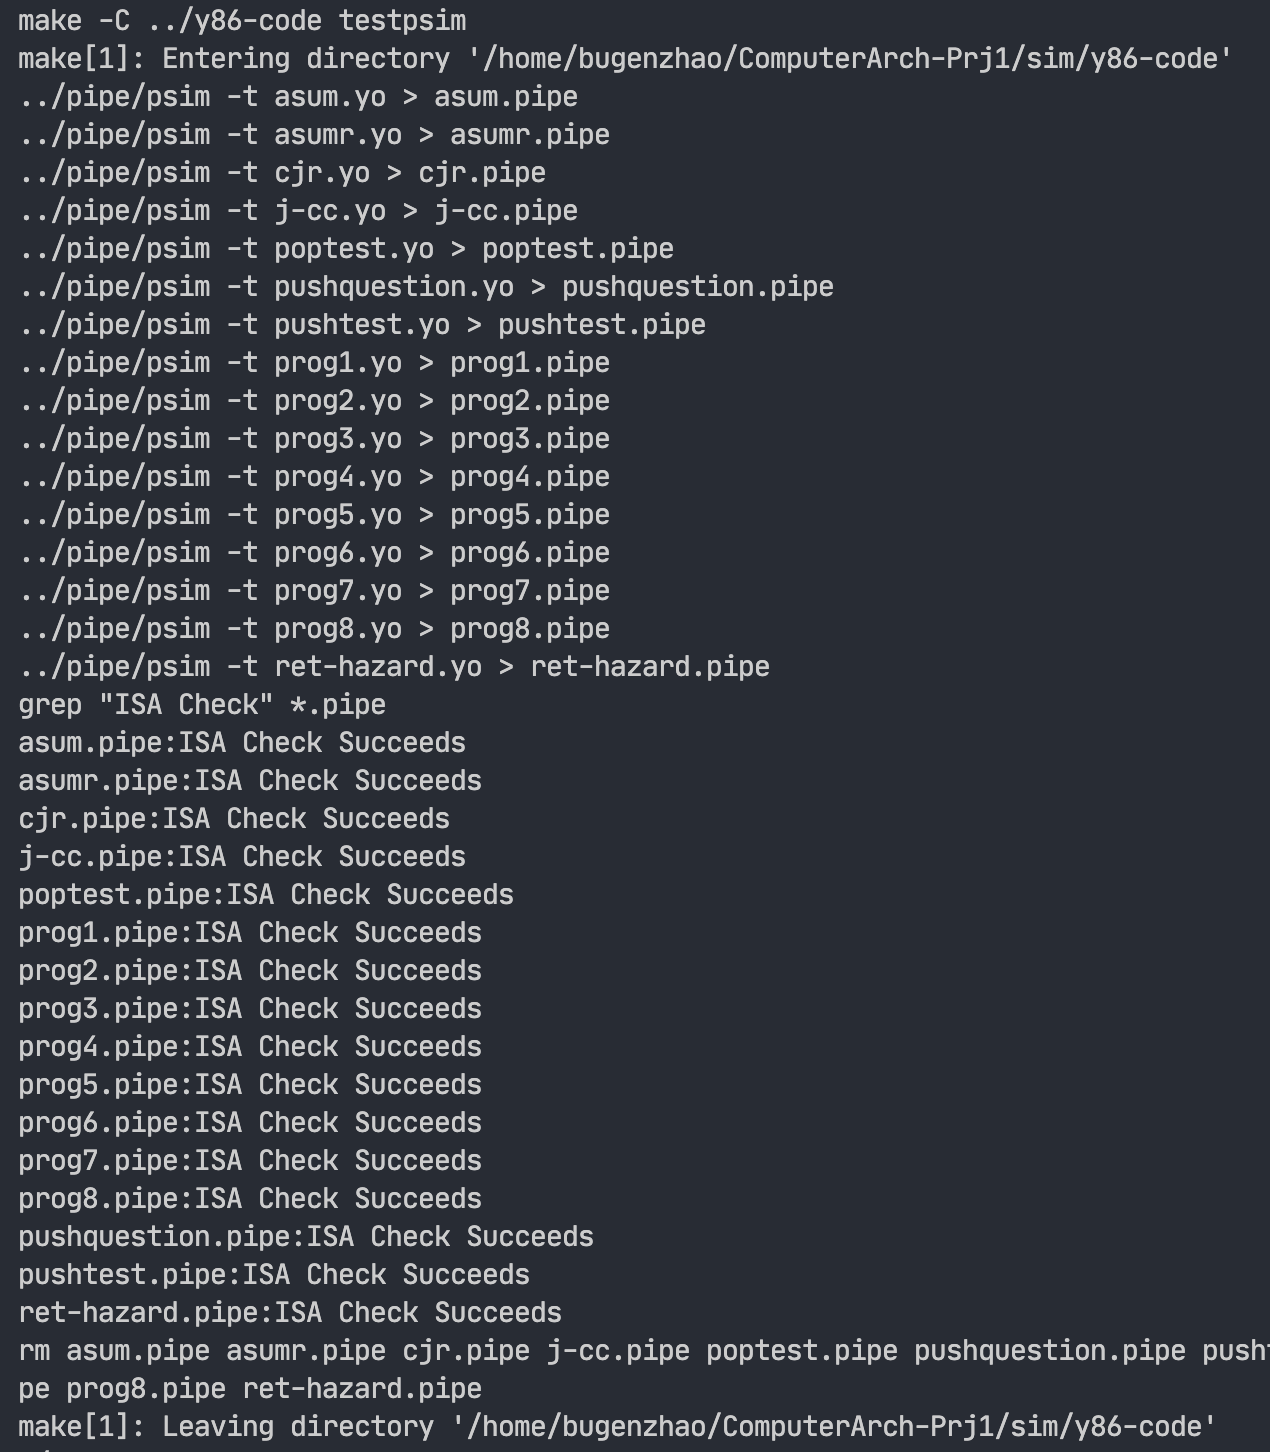
\includegraphics[width=0.9\textwidth]{partC-test2.png} %插入图片,[]中设置图片大小,{}中是图片文件名
        \caption{Part C: benchmark test} %最终文档中希望显示的图片标题
        \label{Fig.partC-benchmark} %用于文内引用的标签
\end{figure}
\begin{figure}[H] %H为当前位置,!htb为忽略美学标准,htbp为浮动图形
        \centering %图片居中
        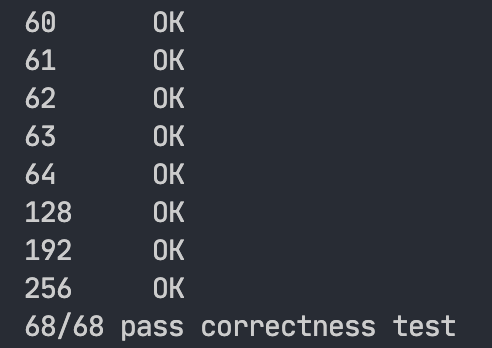
\includegraphics[width=0.4\textwidth]{partC-correctness-test.png} %插入图片,[]中设置图片大小,{}中是图片文件名
        \caption{Part C: correctness test} %最终文档中希望显示的图片标题
        \label{Fig.partC-correctness} %用于文内引用的标签
\end{figure}
\begin{figure}[H] %H为当前位置,!htb为忽略美学标准,htbp为浮动图形
        \centering %图片居中
        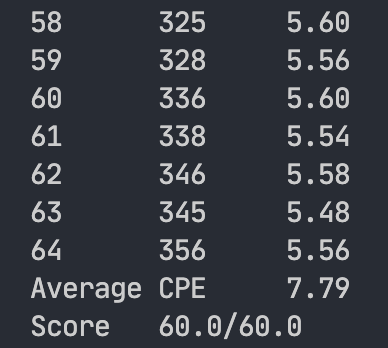
\includegraphics[width=0.4\textwidth]{partC-CPE-test.png} %插入图片,[]中设置图片大小,{}中是图片文件名
        \caption{Part C: CPE test} %最终文档中希望显示的图片标题
        \label{Fig.partC-CPE} %用于文内引用的标签
\end{figure}
\pagebreak
\section{Conclusion}
In this project, we completed the tasks of three parts, which were gradually developed. The first part made us familiar with Y86 assembly syntax, while the second part made us familiar with Y86 SEQ circuit logic, and the third part encouraged us to transform assembly code and Y86 pipeline design.
The following is a summary of the completion of the three parts:
\begin{itemize}
	\item \textbf{Part A}
\begin{itemize}
        \item We write assembly code for three simple functions.
        \item We take care to protect the stack and registers.
        \item We focus on the readability and functional equivalence of the code.
\end{itemize}
	\item \textbf{Part B}
\begin{itemize}
        \item We modify \texttt{SEQ-full.hcl} to add an intruction: \texttt{iaddl}.
\end{itemize}
	\item \textbf{Part C}
\begin{itemize}
        \item We reorder the instructions to avoid hazards.
        \item We do 10-way loop unrolling to speed up the \texttt{while} loop.
        \item We create a search tree to find the number of remaining loops at the minimal cost and then completely unroll the operations for remaining elements.
        \item We modify the \texttt{HCL} file of the pipeline to optimize the branch prediction,  achieving 100\% accuracy for a certain pattern (non-ALU followed by \texttt{jxx}).
\end{itemize}
\end{itemize}
\subsection{Problems}
We've only had some tricky problems in Part C. They are two unsuccessful attempts to modify the pipeline logic to lift the accuracy of branch prediction.
Based on the second attempt, however, we have made some small changes to achieve the goal, which is explained in detail in \textbf{3.2 Achievements}.
\subsubsection{Attempt 1}
In this attempt, we look at a particular code distribution, 
which is "\texttt{andl op1, op2} $\rightarrow$ \texttt{jxx dest}". 
We hope that the branch prediction of \texttt{jxx} under this distribution can reach 100\% accuracy.

The logic is shown in Figure \ref{Fig.partC-attempt1}:
\begin{figure}[H] %H为当前位置,!htb为忽略美学标准,htbp为浮动图形
        \centering %图片居中
        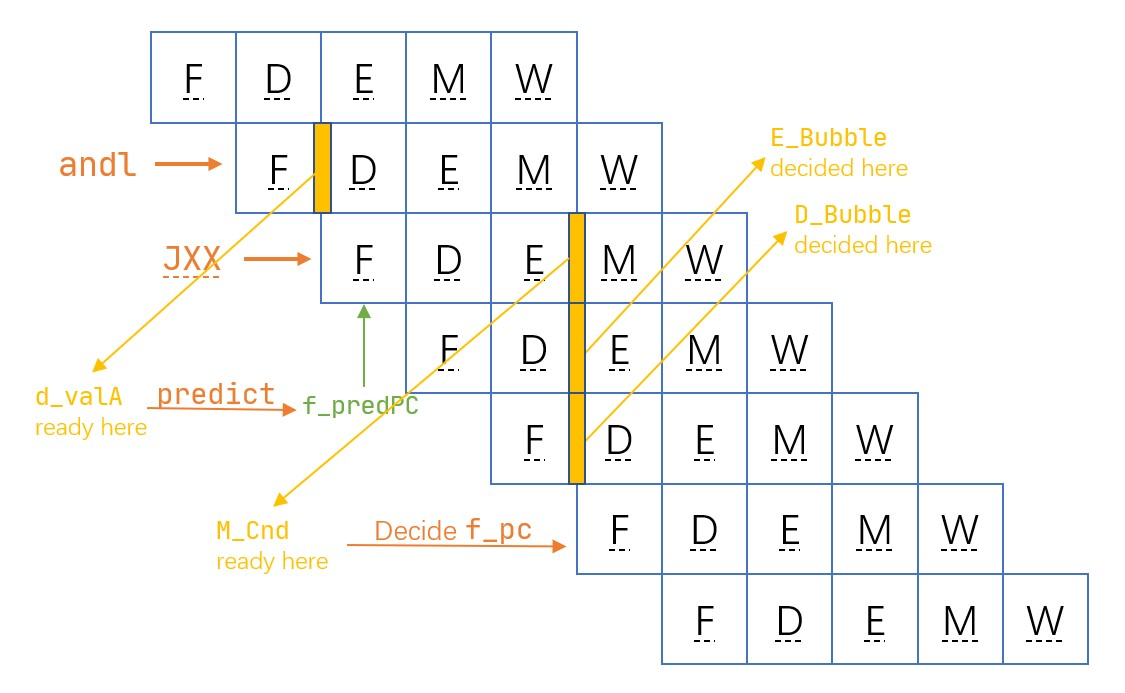
\includegraphics[width=0.7\textwidth]{partC-attempt1.jpg} %插入图片,[]中设置图片大小,{}中是图片文件名
        \caption{Part C: Attempt 1} %最终文档中希望显示的图片标题
        \label{Fig.partC-attempt1} %用于文内引用的标签
\end{figure}
Our initial plan is that, when we detect a \texttt{jxx} after an \texttt{andl}, 
we will do branch prediction according to the value of the first operand of \texttt{andl}. 
Since in our \texttt{ncopy.ys}, there are a lot of this code patterns:
\begin{figure}[H] %H为当前位置,!htb为忽略美学标准,htbp为浮动图形
        \centering %图片居中
        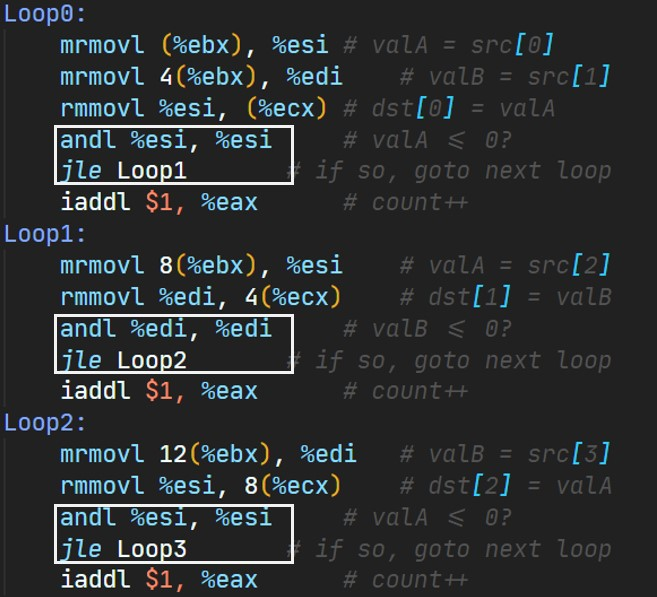
\includegraphics[width=0.6\textwidth]{partC-loop-demo.jpg} %插入图片,[]中设置图片大小,{}中是图片文件名
        \caption{Part C: Loop of Attempt 1} %最终文档中希望显示的图片标题
        \label{Fig.partC-at1-loop} %用于文内引用的标签
\end{figure}
Let's take a closer look at "\texttt{andl op1, op2} $\rightarrow$ \texttt{jxx dest}".

When \texttt{op1 == op2}, i.e., \texttt{rA == rB}, the sign of \texttt{op1} is exactly the sign of \texttt{op1 \& op2}, then we can compare the current conditional jump instruction type with the sign of \texttt{op1} to achieve a 100\% accuracy. 

But if \texttt{op1 != op2}, our prediction will not always succeed, which requires a restore from mispredicted branch, that is, we must find out an approach to determine whether we have mispredicted when the \texttt{jxx} is in MEM stage. However, this is unsolvable since the this information of two register sources has been lost in the pipeline when \texttt{andl} has entered its WB stage.
\subsubsection{Attempt 2}
In this attempt, we look at another code pattern, which is "\texttt{any instruction} $\rightarrow$ \texttt{non-alu instruction} $\rightarrow$ \texttt{jxx dest}", just like the following:
\begin{figure}[H] %H为当前位置,!htb为忽略美学标准,htbp为浮动图形
        \centering %图片居中
        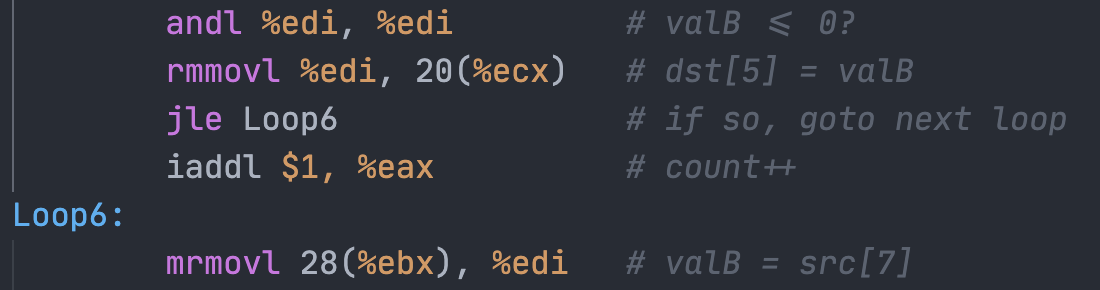
\includegraphics[width=0.7\textwidth]{partC-attempt2.png} %插入图片,[]中设置图片大小,{}中是图片文件名
        \caption{Part C: Attempt 2} %最终文档中希望显示的图片标题
        \label{Fig.partC-attempt2} %用于文内引用的标签
\end{figure}
Since the last instruction of \texttt{jxx} is a non-alu instruction, we are able to get the correct conditional flag when \texttt{jxx} is stll in the Fetch stage. 

Specifically, if the instruction in Execute stage now is a non-alu one, then the current value of \texttt{CC} register will be the correct one for \texttt{jxx}. If the instruction in Execute stage now is an alu one, the the condition flags generated by ALU, i.e. in \texttt{cc\_in}, will be the correct one. 

\textbf{We have ensured that if a non-alu instruction is followed by a \texttt{jxx}, the prediction must be correct.} Thus, when we are processing with the logic of restoring form misprediction, we only need to focus on the case where the previous instruction of \texttt{jxx} is an alu instruction. According to this, we avoid the problems we encountered in our first attempt, since it is really easy to get the \texttt{ifun} field and decide the type of an instruction in Write-back stage.

However, when we finished the implementation in \texttt{HCL} file, \textbf{a strange problem arose}. The simulator using this branch prediction approach can pass all the ISA tests provided, but yielded a large number of "bad count" in \texttt{ncopy.ys}. 

It took us about six hours to troubleshoot the problem and finally pin down the cause of the problem into two signals in the pipeline simulator: \textbf{\texttt{cc\_in} and \texttt{e\_valE}}. Please refer to the next section on how we finally solved this problem.
\subsection{Achievements}
\subsubsection{A Successful Attempt 3}
For the "bad count" problems, we explored for a long time and finally realized that when we predicted the branch, \textbf{the simulator may not generate the correct ALU output values}, say, \texttt{e\_valE} and \texttt{cc\_in}. After a talk with Chi Zhang, we adopted a compromise method, that is, manually call the C function in the simulator program to generate a correct ALU output, and take this as the basis of prediction. It finally succeeded and leaded to a CPE of $7.79$.

\begin{lstlisting}
# For JXX in ID and ALU in EX, check the cc generated by ALU
# Note that the simulator do not generate `cc_in` correctly
boolsig f_cnd_alu 
        'cond_holds(compute_cc(id_ex_curr->ifun, 
                    gen_aluA(), gen_aluB()), 
                    if_id_next->ifun)'
\end{lstlisting}

In this case, we seem to predict the branch by doing complex operations in the Fetch stage, which also seems unreasonable in real pipelined processor design. However, according to the characteristics of the logic circuit, all signals in the circuit must be able to reach steady state in one clock cycle, so the output of ALU must be correct. \textbf{We don't need to add any additional complex hardware in the Fetch stage to perform such a prediction policy. We just need a simple unit instead to compare the \texttt{ifun} of the current \texttt{jxx} instruction with the three flags of \texttt{zf}, \texttt{sf} and \texttt{of} in \texttt{cc} or \texttt{cc\_in}}, which is similar to the technique named "delayed slot" and is a fairly practical design in fact. 

\subsubsection{Performance Improvement}
By modifying the pipeline logic, we managed to accelerate the program to a very surprising degree:
$$
        \text{CPE} = 12.98 \rightarrow \text{CPE} = 9.83 \rightarrow \text{CPE} = 8.95 \rightarrow {\color{blue}\textbf{CPE }\mathbf{= 7.79}}
$$

We even try to unlimit the number of the array size. By modifying \texttt{benchmark.pl}, 
we push the upper bound to be 400 to test the best performance of our implementation (see Figure \ref{Fig.partC-limit}).
\begin{figure}[H] %H为当前位置,!htb为忽略美学标准,htbp为浮动图形
        \centering %图片居中
        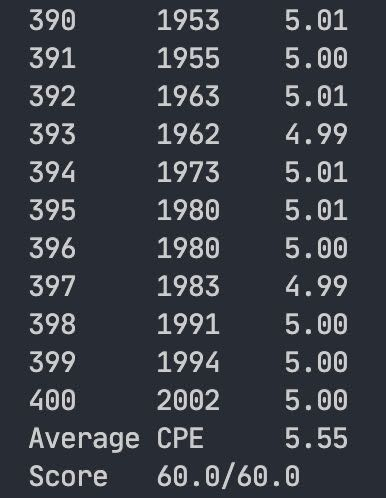
\includegraphics[width=0.4\textwidth]{partC-larger-scale-test.jpg} %插入图片,[]中设置图片大小,{}中是图片文件名
        \caption{Part C: larger scale test} %最终文档中希望显示的图片标题
        \label{Fig.partC-limit} %用于文内引用的标签
\end{figure}
From analysis, we could safely estimate that the theoretical minimum CPE should be around $4.5$ to $5.0$. \textbf{So it's almost certain that the optimizations we've done under the existing ISA framework are close to extreme.}
\subsubsection{Code readability}
We put a lot of effort into the readability of the code for parts A.
\begin{itemize}
        \item For functions that contain loops, we can always break it down into three logical regions: \texttt{loop}, \texttt{test}, and \texttt{return}.
        \item For various registers, we always annotate its purpose with comments
        \item For code that's not so obvious, we always leave the comment showing its counterpart in the C function next to it.
\end{itemize}

We have also left understandable and sufficient comments in the header of the modified files in Part B and Part C. Please refer to \texttt{ncopy.ys}, \texttt{pipe-full.hcl}, \texttt{pipe-zzcc.hcl}, and \texttt{seq-full.hcl}.

\subsection{Feelings}
This is a very interesting and valuable project, and we have worked together perfectly. 
When Ziqi achieved full score for Part C in two hours, we started thinking about whether we could get CPE down to the limitation.
We ended up spending two days talking, drawing, and writing code to test.
But the most exciting thing was that after two big failures, we finally got there in a very "weird" way.
It should be noted, however, that there is an inherent problem with the simulator for the pipeline processor. 
Otherwise our second attempt should have been successful and would not have required special means to implement it in the third attempt.

This project allowed us to reap the valuable sense of accomplishment brought by not giving up. We are also very grateful to have been able to take this course and to be introduced to such a valuable project.

Finally, we would like to specially thank Miss Shen and the TAs for their instruction and support, so that we can successfully complete this project.
%----------------------------------------------------------------------------------------
\end{document}